\documentclass[
	11pt, % Set the default font size, options include: 8pt, 9pt, 10pt, 11pt, 12pt, 14pt, 17pt, 20pt
	%t, % Uncomment to vertically align all slide content to the top of the slide, rather than the default centered
	%aspectratio=169, % Uncomment to set the aspect ratio to a 16:9 ratio which matches the aspect ratio of 1080p and 4K screens and projectors
]{beamer}

\graphicspath{{images/}{./}} % Specifies where to look for included images (trailing slash required)

\usepackage{booktabs} % Allows the use of \toprule, \midrule and \bottomrule for better rules in tables
\usetheme{Madrid}
\useinnertheme{circles}

%----------------------------------------------------------------------------------------
%	SELECT FONT THEME & FONTS
%----------------------------------------------------------------------------------------

% Beamer comes with several font themes to easily change the fonts used in various parts of the presentation. Review the comments beside each one to decide if you would like to use it. Note that additional options can be specified for several of these font themes, consult the beamer documentation for more information.

\usefonttheme{default} % Typeset using the default sans serif font
%\usefonttheme{serif} % Typeset using the default serif font (make sure a sans font isn't being set as the default font if you use this option!)
%\usefonttheme{structurebold} % Typeset important structure text (titles, headlines, footlines, sidebar, etc) in bold
%\usefonttheme{structureitalicserif} % Typeset important structure text (titles, headlines, footlines, sidebar, etc) in italic serif
%\usefonttheme{structuresmallcapsserif} % Typeset important structure text (titles, headlines, footlines, sidebar, etc) in small caps serif

%------------------------------------------------

%\usepackage{mathptmx} % Use the Times font for serif text
%\usepackage{palatino} % Use the Palatino font for serif text

%\usepackage{helvet} % Use the Helvetica font for sans serif text
%\usepackage[default]{opensans} % Use the Open Sans font for sans serif text
%\usepackage[default]{FiraSans} % Use the Fira Sans font for sans serif text
%\usepackage[default]{lato} % Use the Lato font for sans serif text
\usepackage{chemformula}
\usepackage[T1]{fontenc}

%----------------------------------------------------------------------------------------
%	PRESENTATION INFORMATION
%----------------------------------------------------------------------------------------

\title[Utylizacja akumulatorów]{Utylizacja akumulatorów} % The short title in the optional parameter appears at the bottom of every slide, the full title in the main parameter is only on the title page

\subtitle{Budowa, degradacja i odzyskiwanie ogniw} % Presentation subtitle, remove this command if a subtitle isn't required

\author[P. Niedźwiedziński]{Patryk Niedźwiedziński}

\institute[PUT]{Politechnika Poznańska \\ \smallskip Wydział Inżynierii Środowiska i Energetyki} 

\date[16.11.2022]{Chemia \\ 16 listopada 2022}

%----------------------------------------------------------------------------------------

\begin{document}

%----------------------------------------------------------------------------------------
%	TITLE SLIDE
%----------------------------------------------------------------------------------------

\begin{frame}
	\titlepage % Output the title slide, automatically created using the text entered in the PRESENTATION INFORMATION block above
\end{frame}

%----------------------------------------------------------------------------------------
%	TABLE OF CONTENTS SLIDE
%----------------------------------------------------------------------------------------

% The table of contents outputs the sections and subsections that appear in your presentation, specified with the standard \section and \subsection commands. You may either display all sections and subsections on one slide with \tableofcontents, or display each section at a time on subsequent slides with \tableofcontents[pausesections]. The latter is useful if you want to step through each section and mention what you will discuss.

\begin{frame}
	\frametitle{Spis treści} % Slide title, remove this command for no title
	
	\tableofcontents % Output the table of contents (all sections on one slide)
	%\tableofcontents[pausesections] % Output the table of contents (break sections up across separate slides)
\end{frame}

%----------------------------------------------------------------------------------------
%	PRESENTATION BODY SLIDES
%----------------------------------------------------------------------------------------

\section{Budowa ogniw}

\subsection{Rodzaje ogniw}
%------------------------------------------------

\begin{frame}
	\centering
  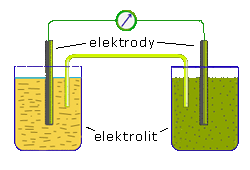
\includegraphics[width=8cm]{ogniwo.png}
\end{frame}

\begin{frame}{Lampa ogrodowa z Lidla}{Ogniwo wodorkowe: Ni-MH}
  \centering
  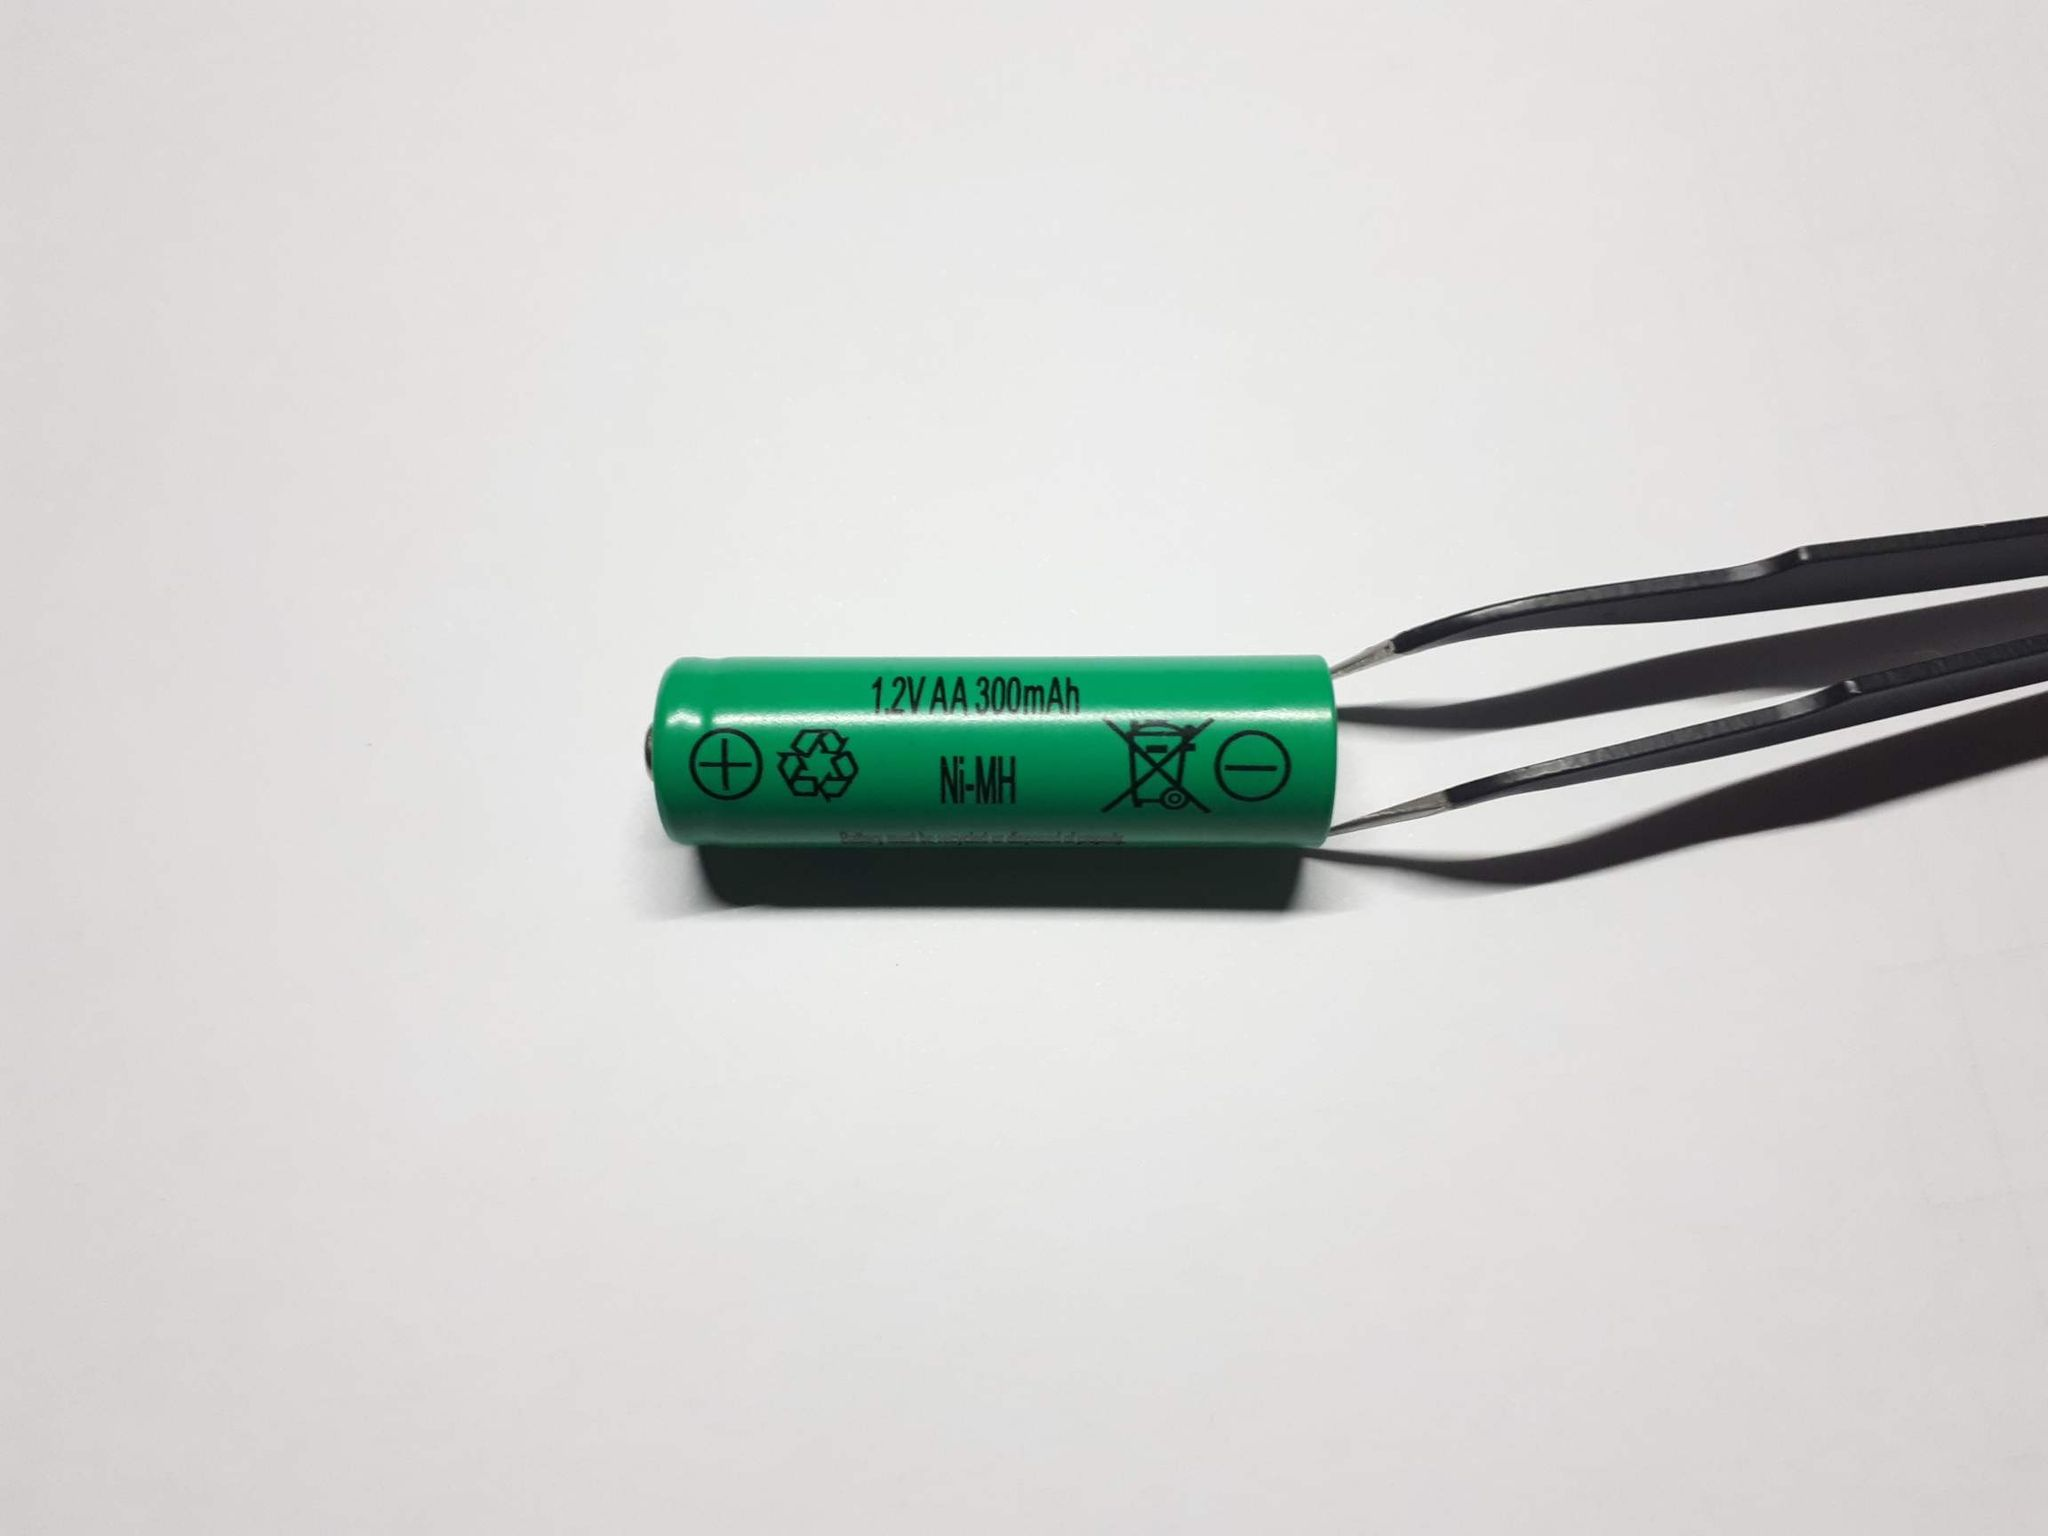
\includegraphics[width=8cm]{solar-lamp.jpg}
	
	%\ch{Ni} - katoda, \ch{M (LaNi5)} - anoda, stop metali chłonący wodór, \ch{H(H2O + KOH)}\cite{c05}.

\end{frame}

\begin{frame}{Słuchawki Bluetooth}{Bateria litowa: Li-ion}
  \centering
  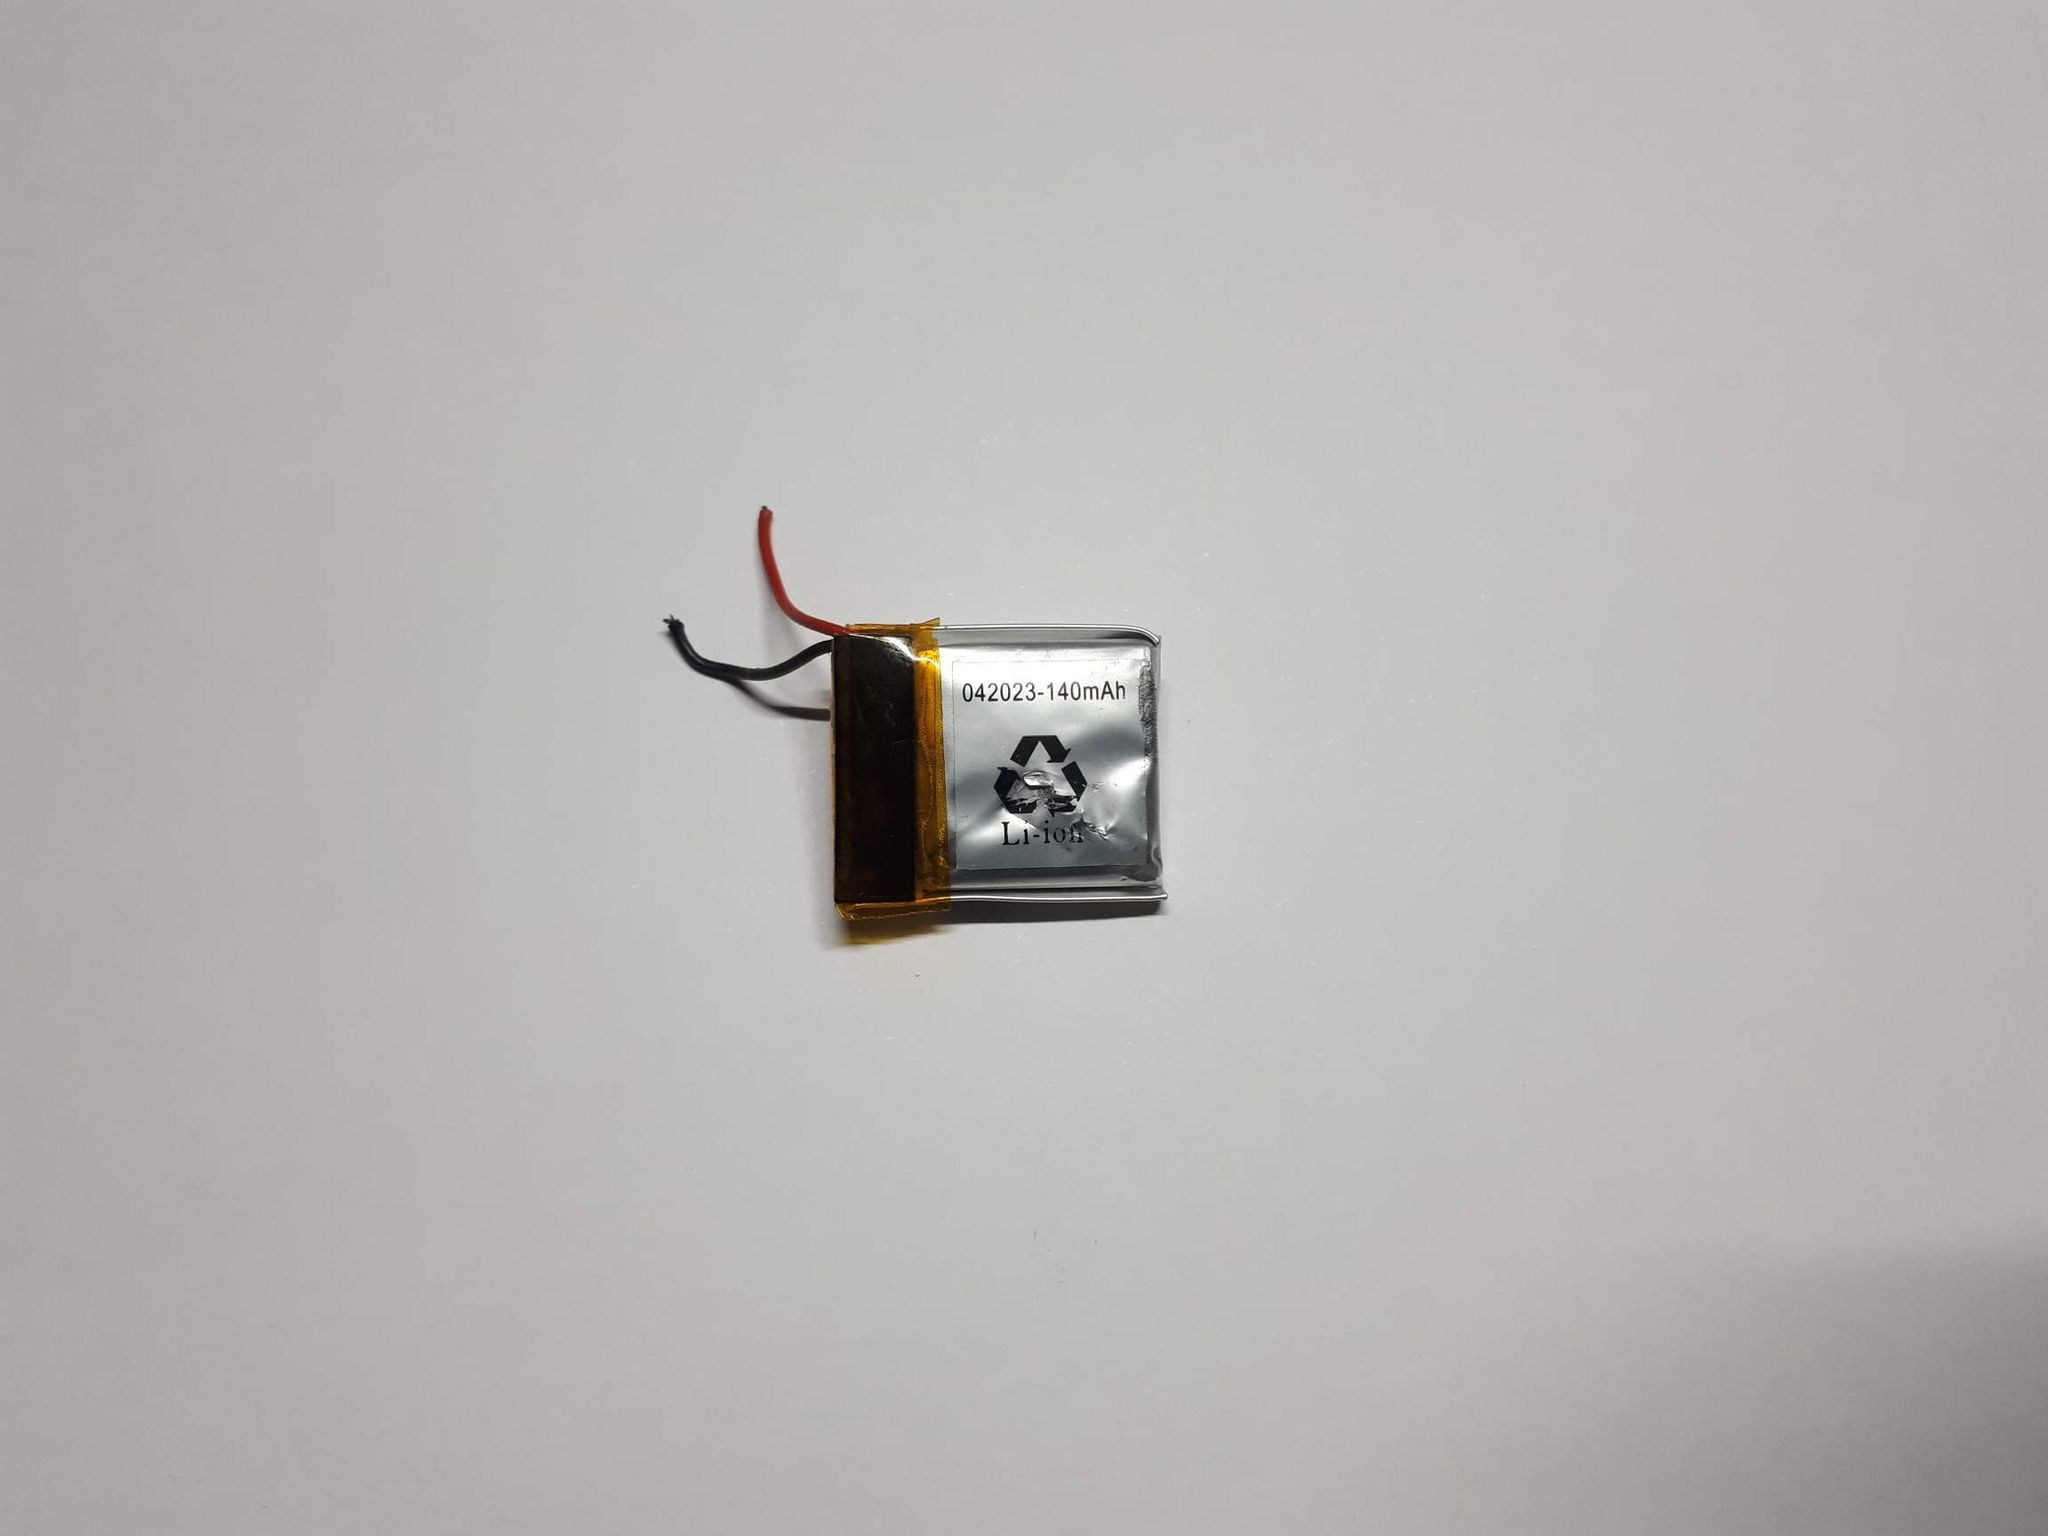
\includegraphics[width=8cm]{earbuds.jpg}
	
\end{frame}

\begin{frame}{Bank energii}{Akumulator kwasowo-ołowiowy: Pb}
  \centering
  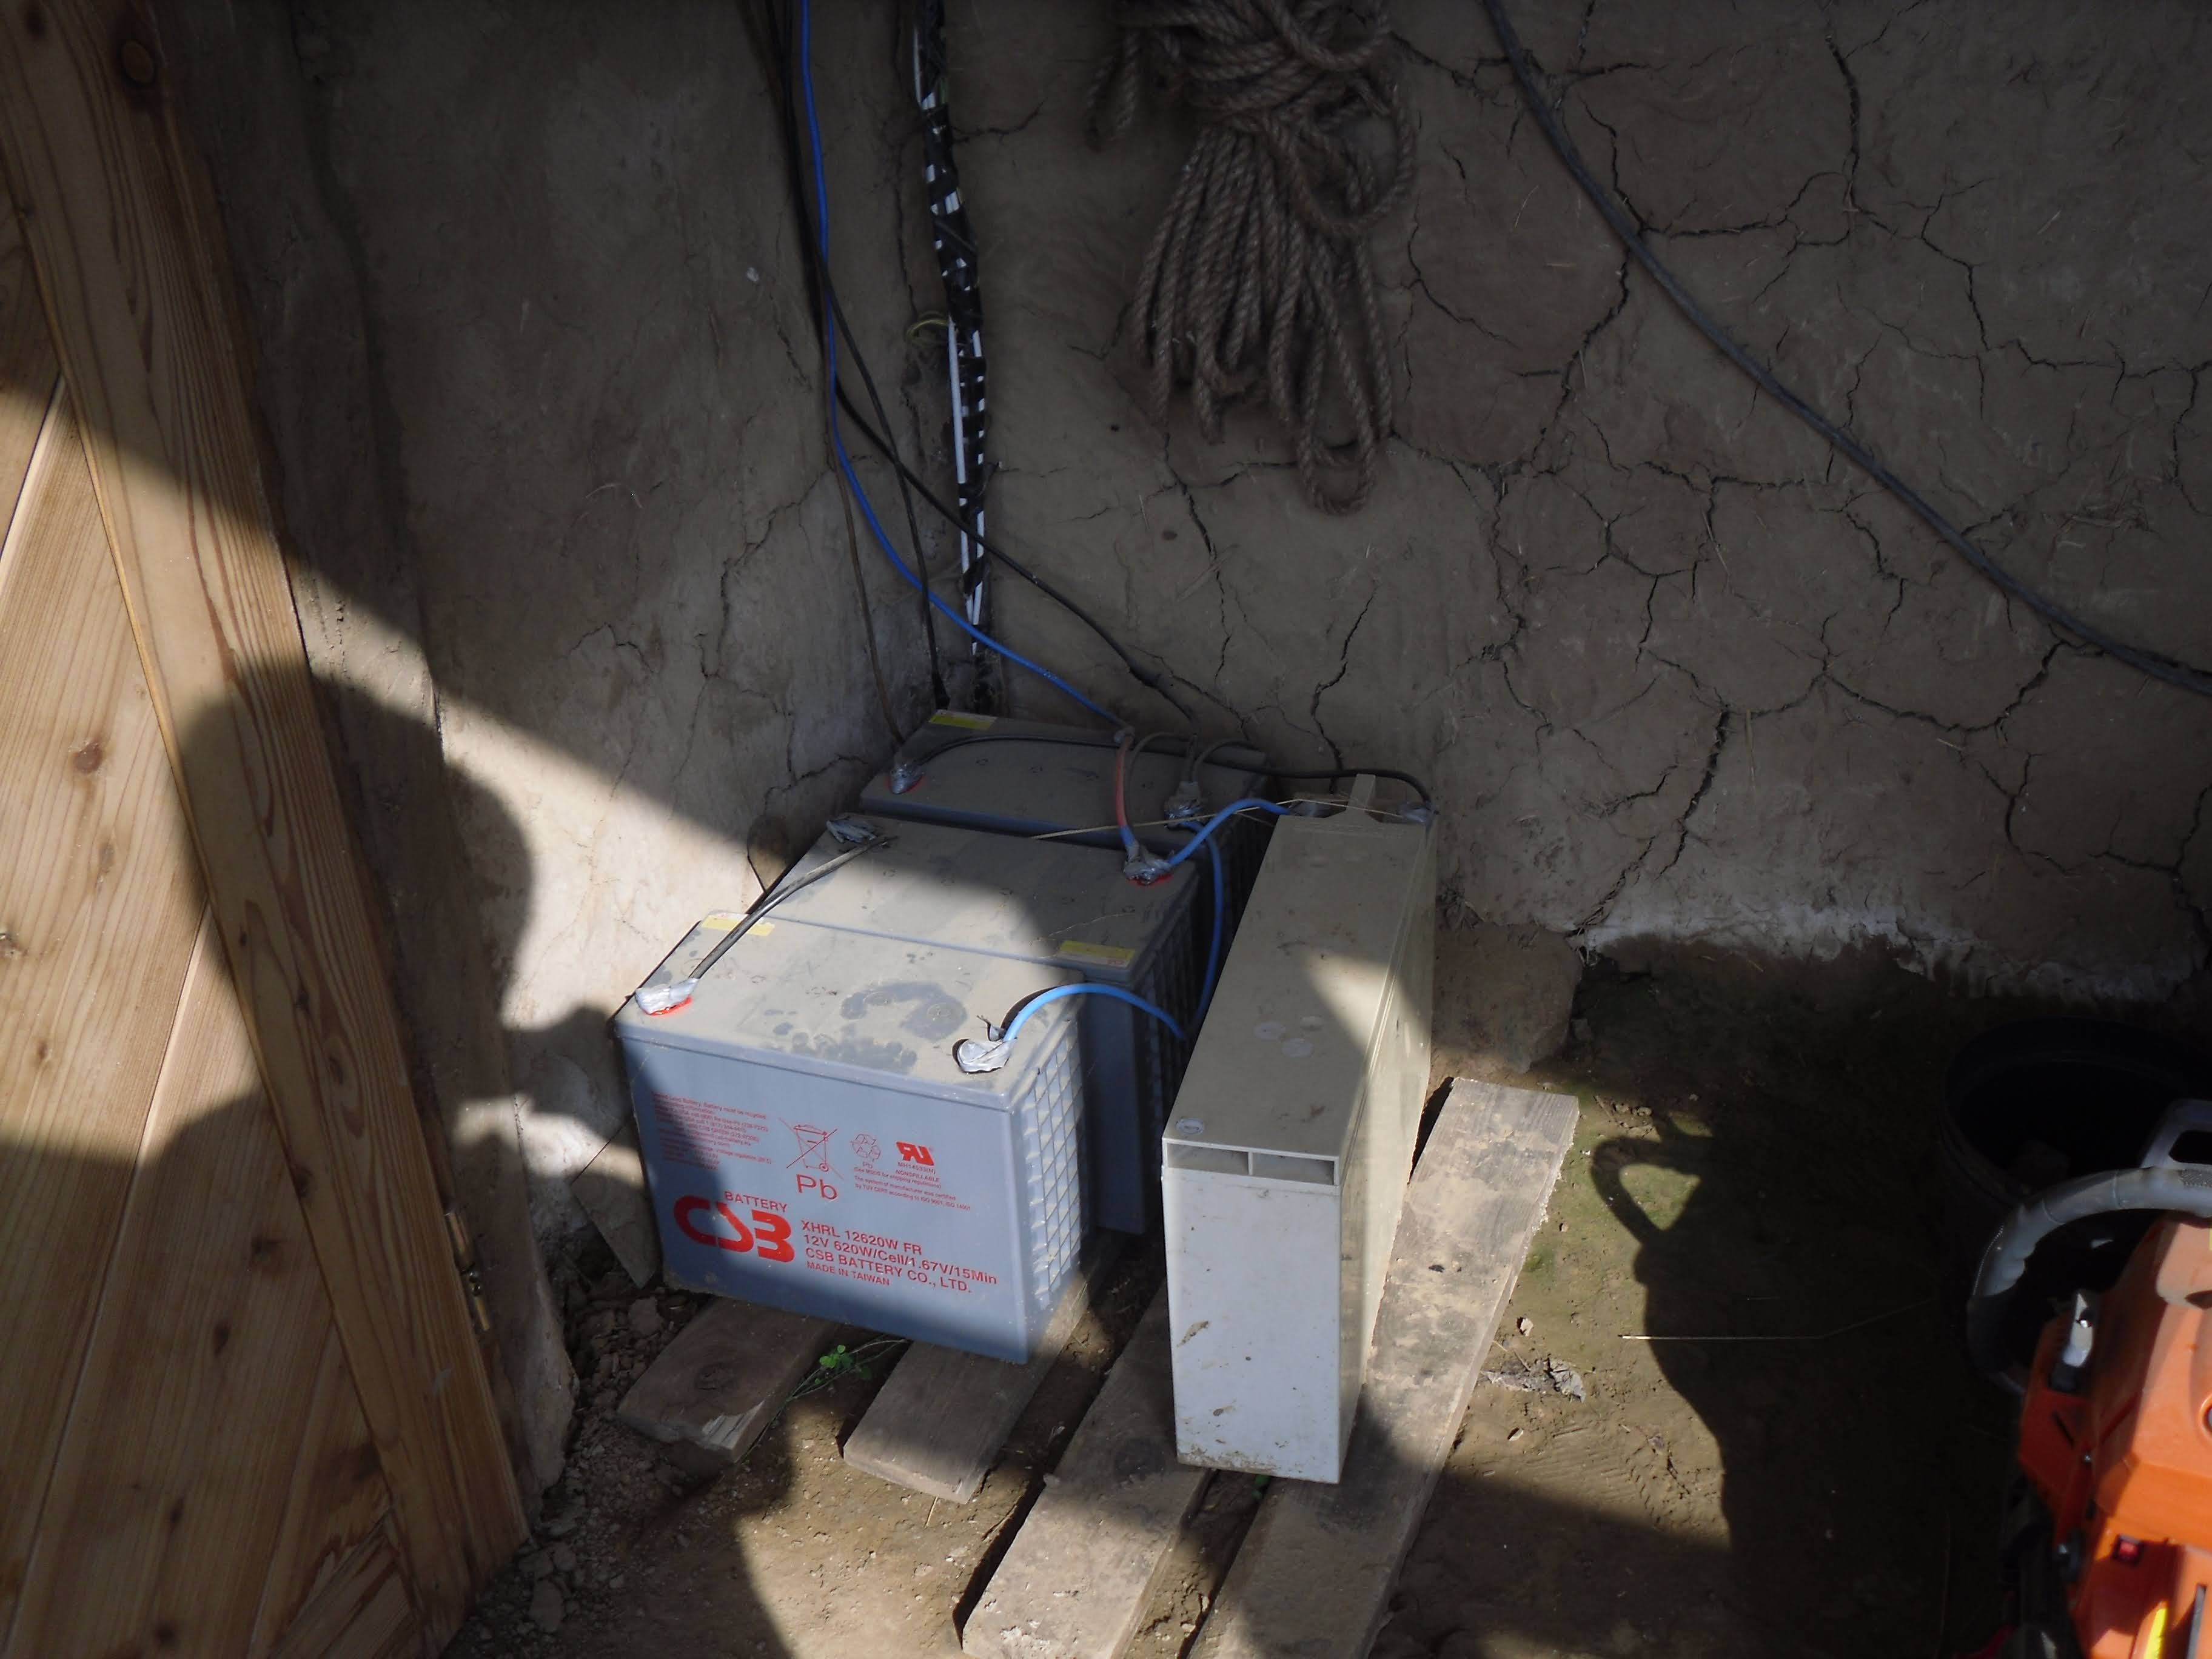
\includegraphics[width=8cm]{lead-acid.jpg}

	%\ch{Pb} - katoda, \ch{PbO2} - anoda, \ch{H2SO4} - elektrolit (kwas siarkowy)
\end{frame}

\begin{frame}{Wiertarka}{Akumulator niklowo-kadmowy: Ni-Cd}
  \centering
  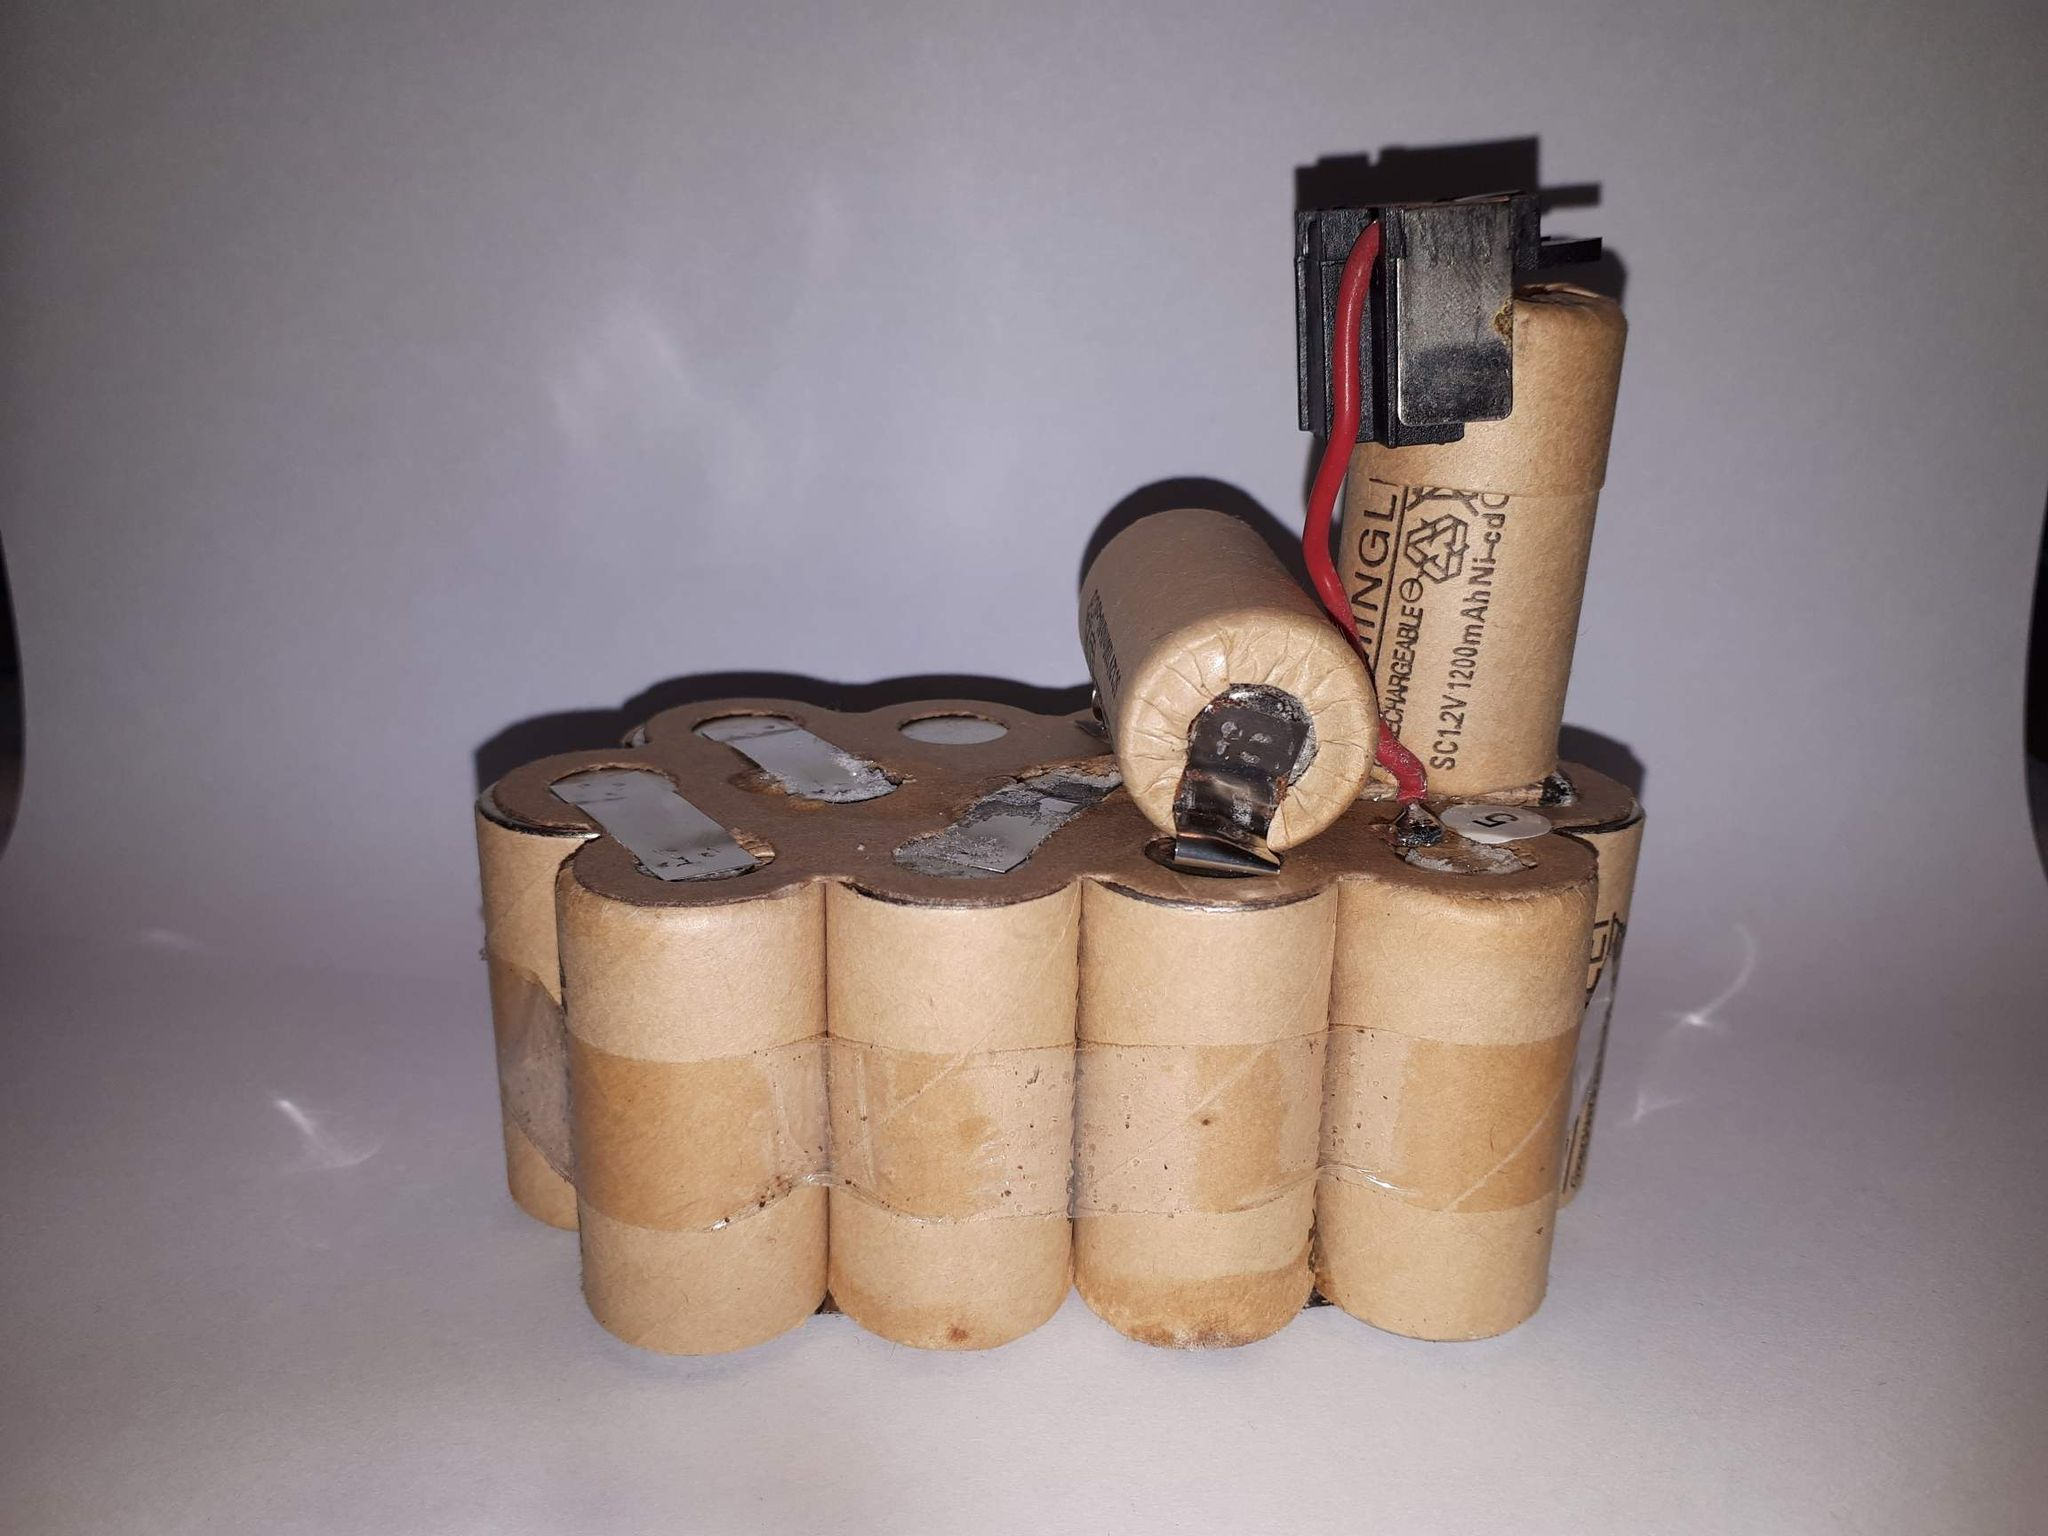
\includegraphics[width=8cm]{drill.jpg}

	%\ch{Cd} - anoda, \ch{NiOOH} - katoda, \ch{KOH} - elektrolit
\end{frame}

\begin{frame}{Nokia 8810}{Li-ion}

  \centering
  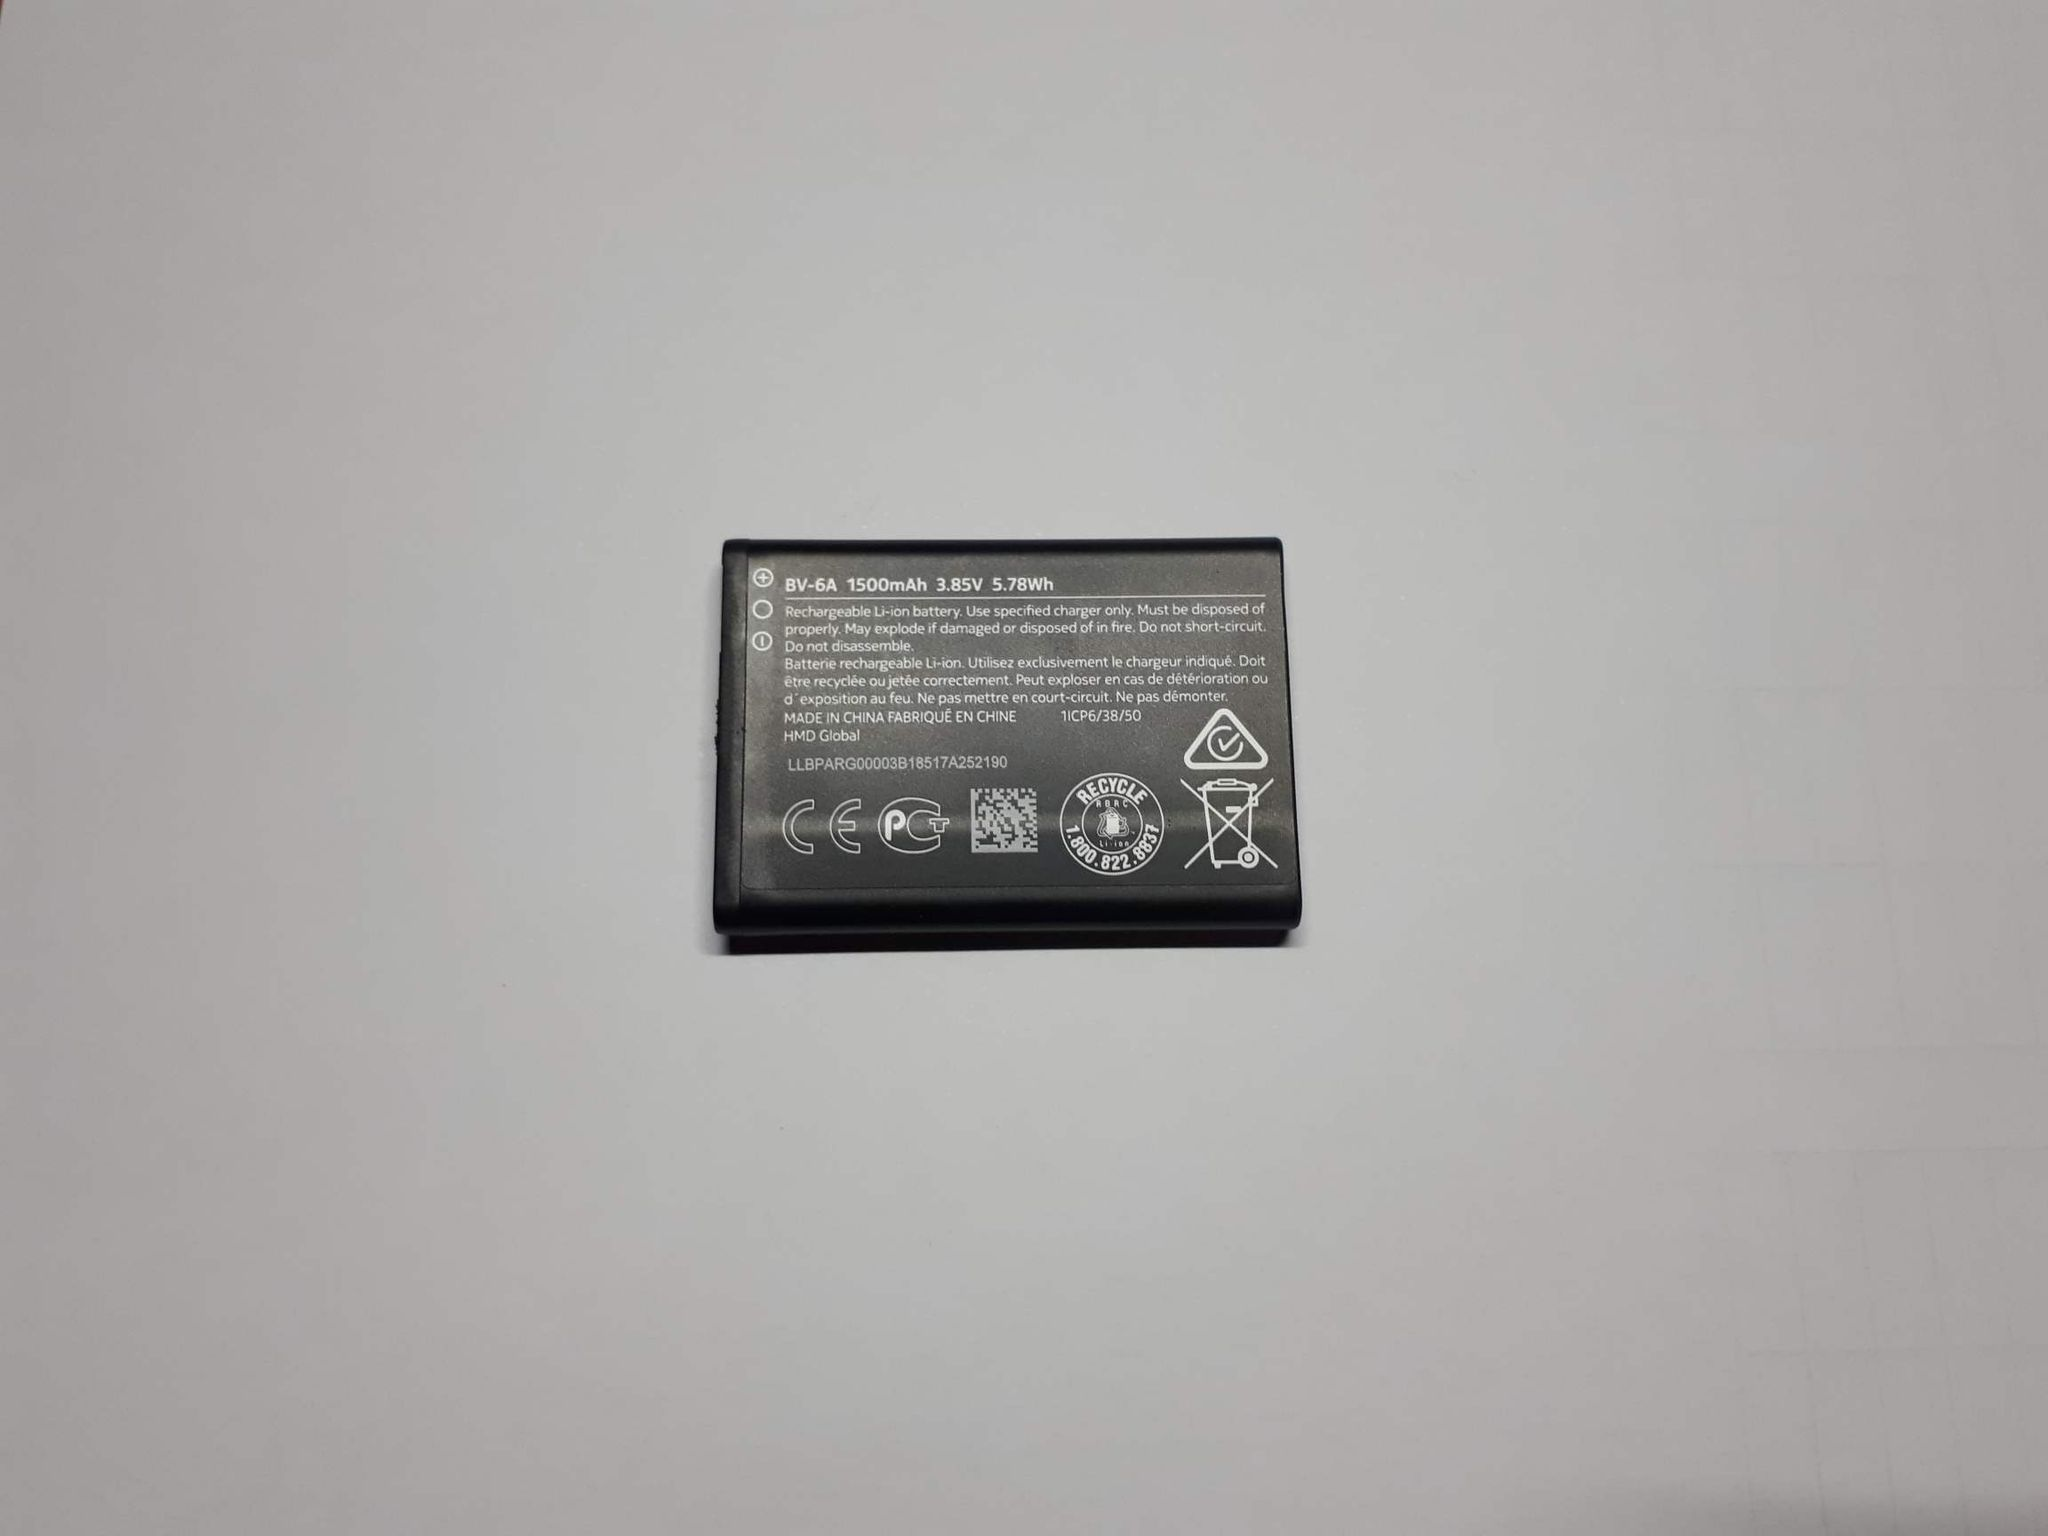
\includegraphics[width=8cm]{phone.jpg}

	\ch{Li}* - elektrolit, \ch{LiMnO4} - katoda, Grafit - anoda\cite{c05}\cite{m14}.
\end{frame}

\begin{frame}{18650}{Li-ion}

  \centering
  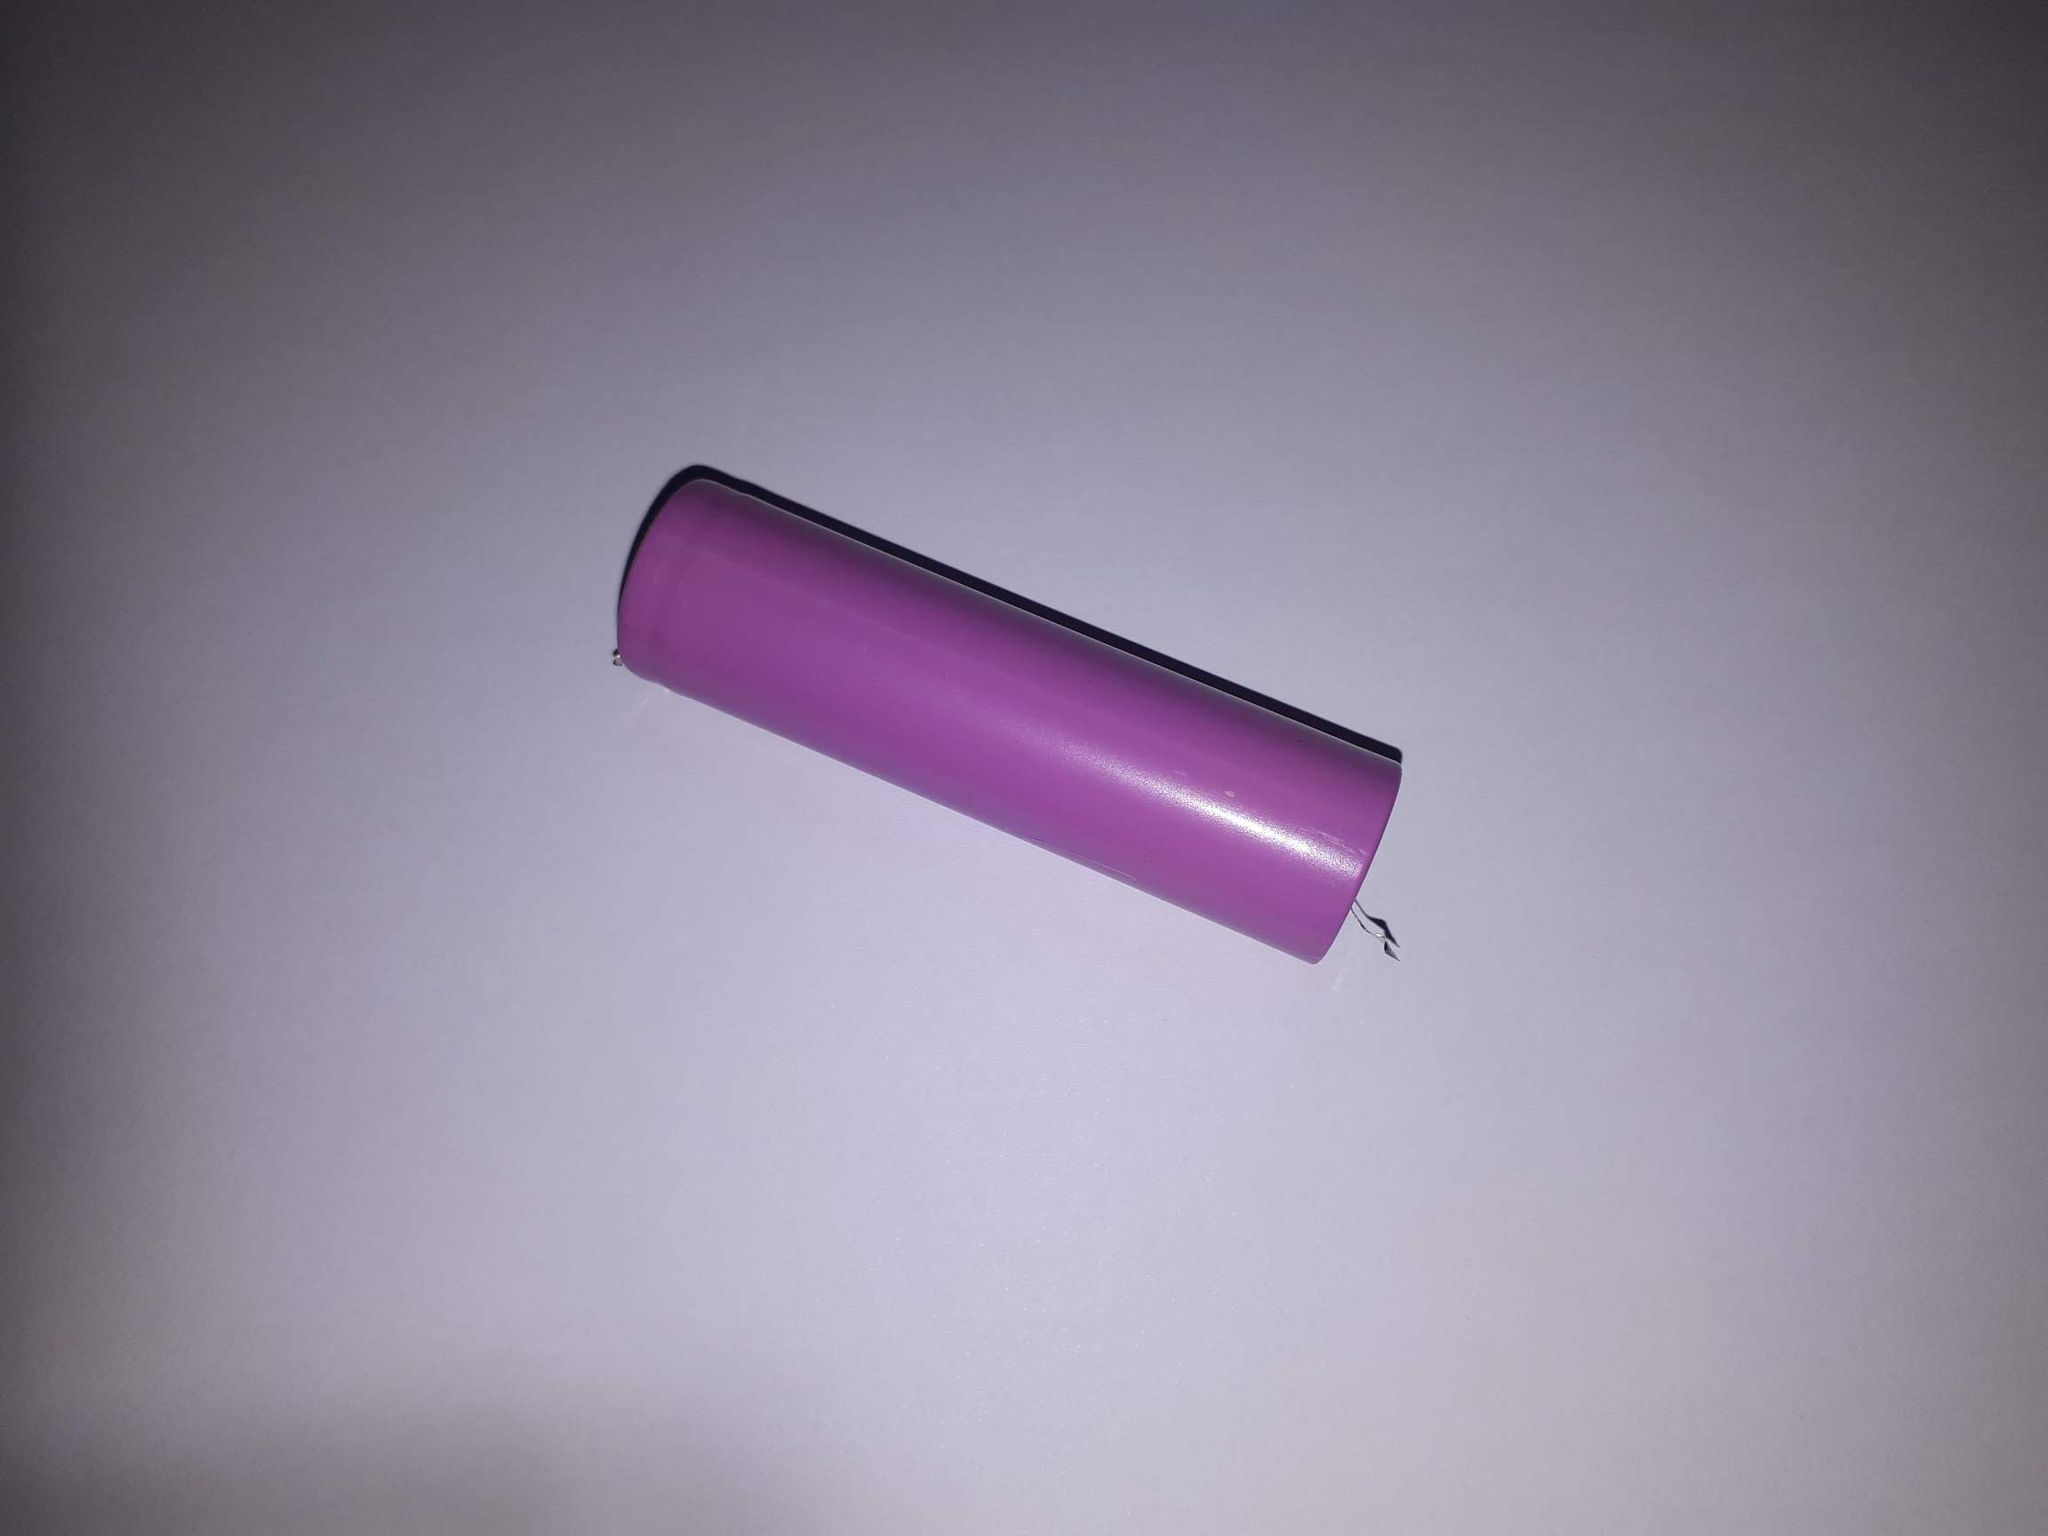
\includegraphics[width=8cm]{18650.jpg}
\end{frame}

\section{Degradacja akumulatora}

\subsection{Działanie akumulatora Li-ion}

\begin{frame}
	\frametitle{Działanie akumulatora Li-ion}
	\centering
	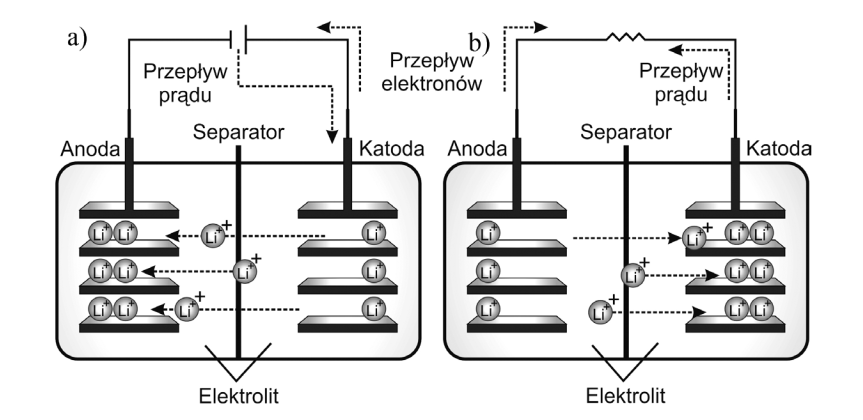
\includegraphics[width=9cm]{liion.png}\cite{m14}
\end{frame}

\subsection{Degradacja}

\begin{frame}
  \centering
	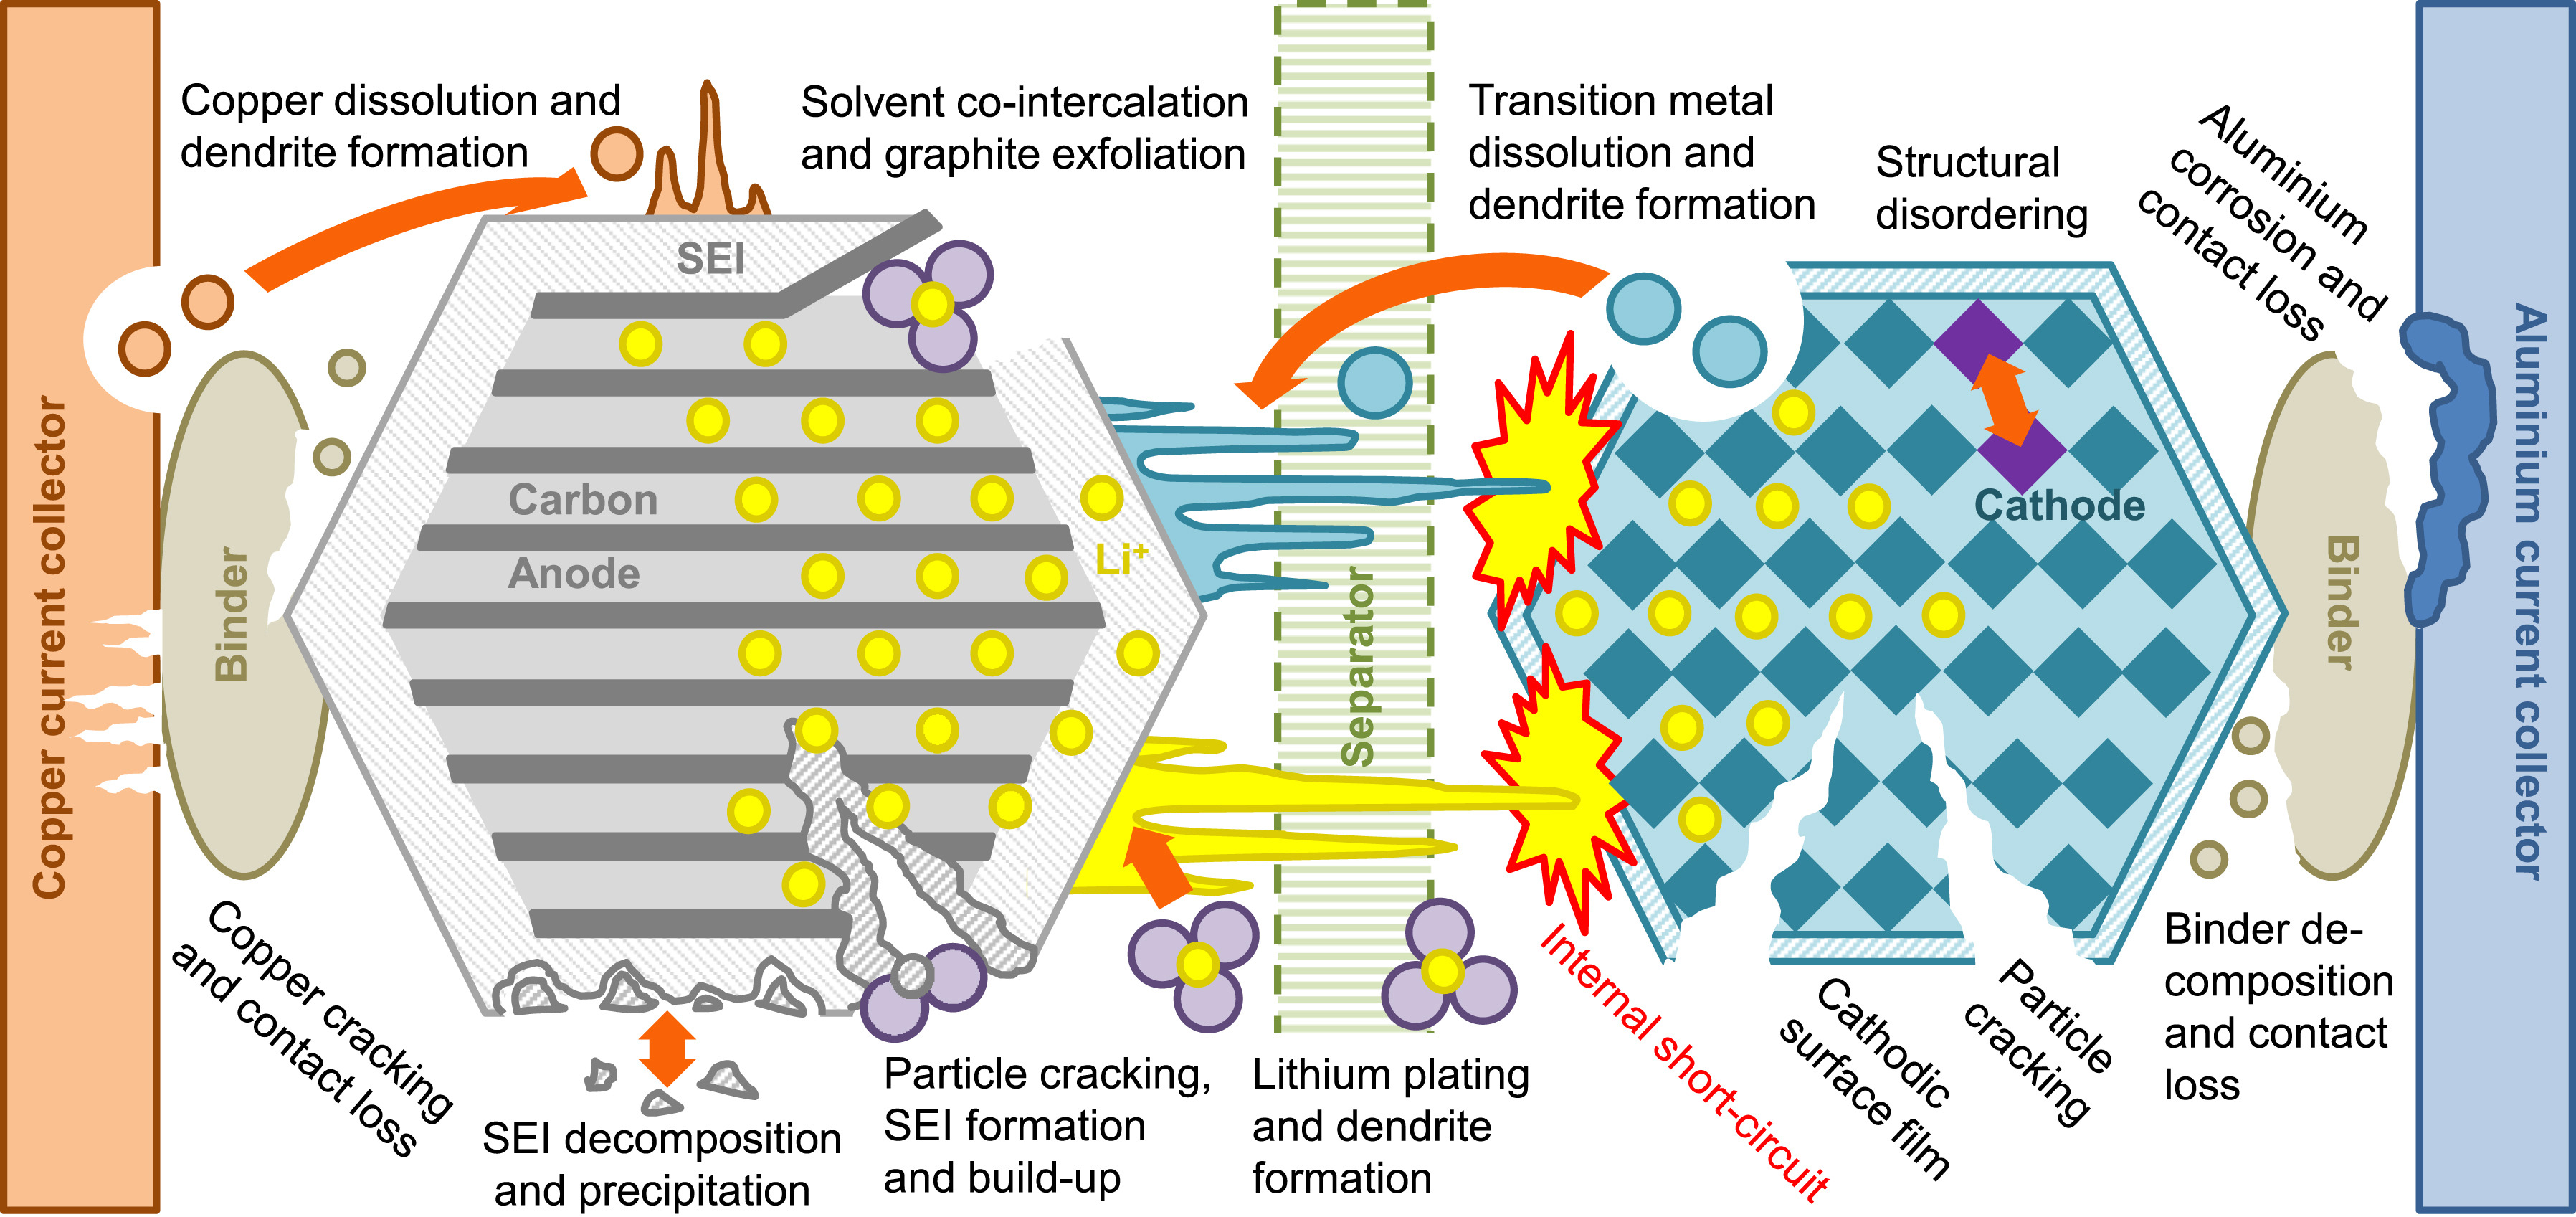
\includegraphics[width=12cm]{degradation-all.jpg}\cite{b17}
\end{frame}

\begin{frame}
	\frametitle{Degradacja}
	\centering
	\begin{itemize}
		\item Utrata dostępnych jonów litu
		\item Utrata materiału na anodzie
		\item Utrata materiału na katodzie
	\end{itemize} \cite{b17}

	\vspace{4em}
	Trudno jest określić "stan zdrowia" baterii \cite{s21}

\end{frame}

\section{Koniec życia akumulatora}

\begin{frame}
	\frametitle{Sprzedaż akumulatorów na świecie}
	\centering
	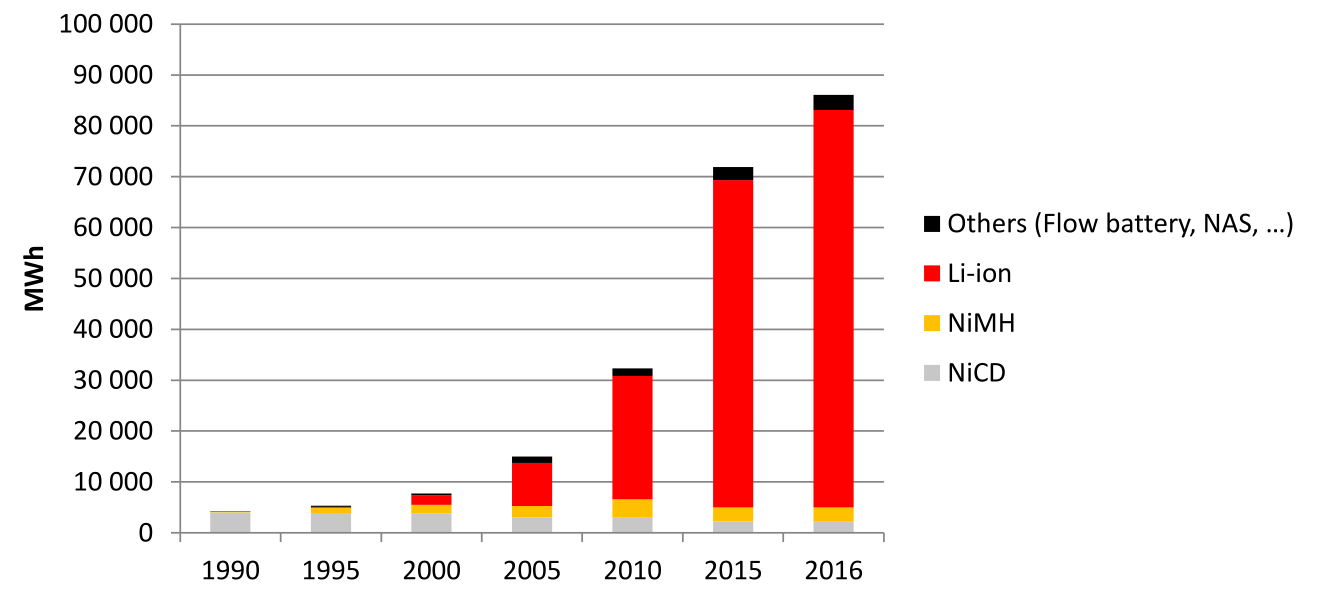
\includegraphics[width=10cm]{sales.png}\cite{p17}
	$$ 80\ 000 MWh \div 140 \frac{Wh}{kg} \approx 570\ 000 t$$\cite{m14}
\end{frame}

\begin{frame}
	\frametitle{Wcale nie na śmietnik}
	\centering
	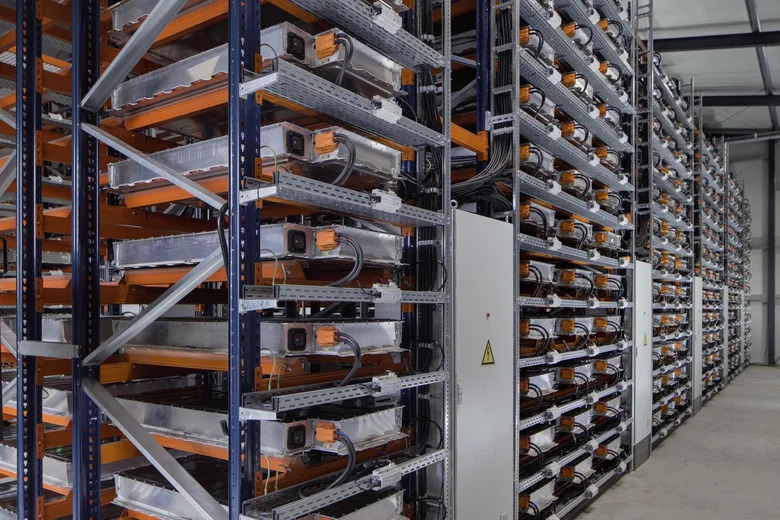
\includegraphics[width=8cm]{bmw.jpg}

	Stacjonarny magazyn energii z używanych baterii elektryków BMW\cite{c17}
\end{frame}

	\begin{frame}
	\centering
	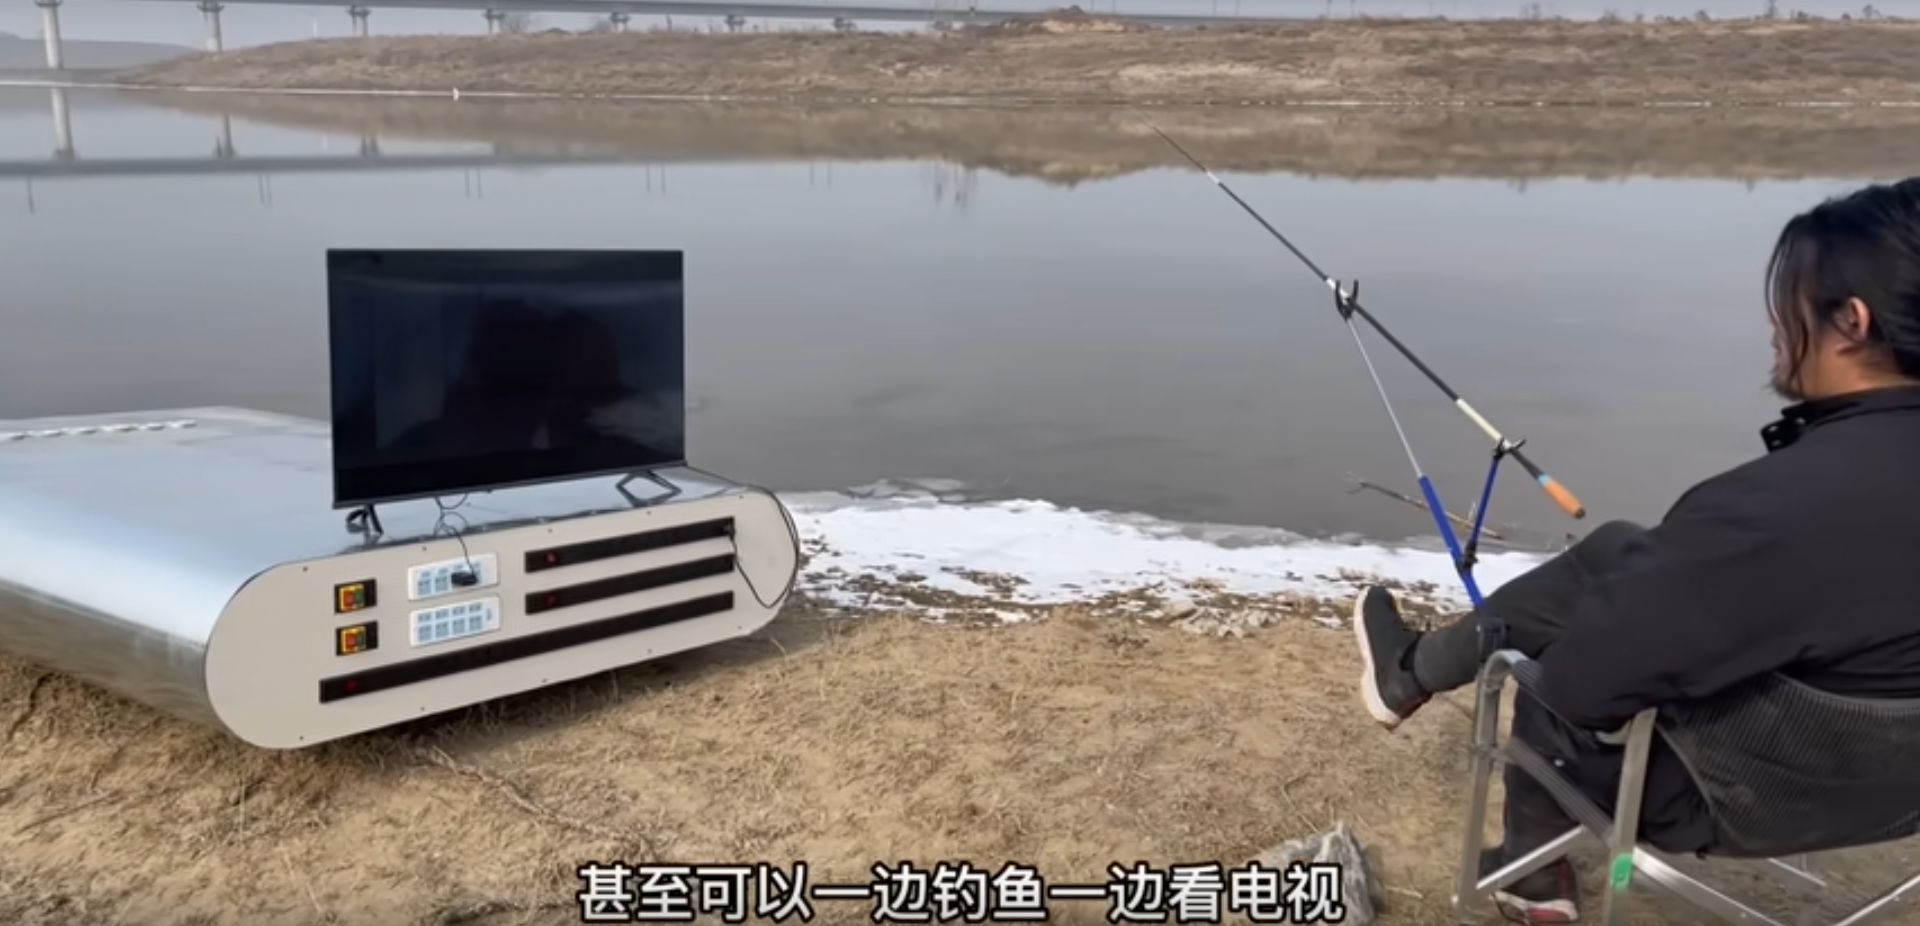
\includegraphics[width=10cm]{big-powerbank.png}
	https://www.youtube.com/watch?v=-oilA8nLfsk
	\end{frame}

\begin{frame}
	\frametitle{Utylizacja zużytych akumulatorów}

	\begin{enumerate}
		\item Zmielenie akumulatora (w całości lub w częściach)
		\item Proces oddzielenia materiałów
		\begin{itemize}
			\item pirometalurgia
			\item hydrometalurgia
			\item bio-hydrometalurgia
		\end{itemize}
	\end{enumerate}
\end{frame}

\begin{frame}
	\centering
	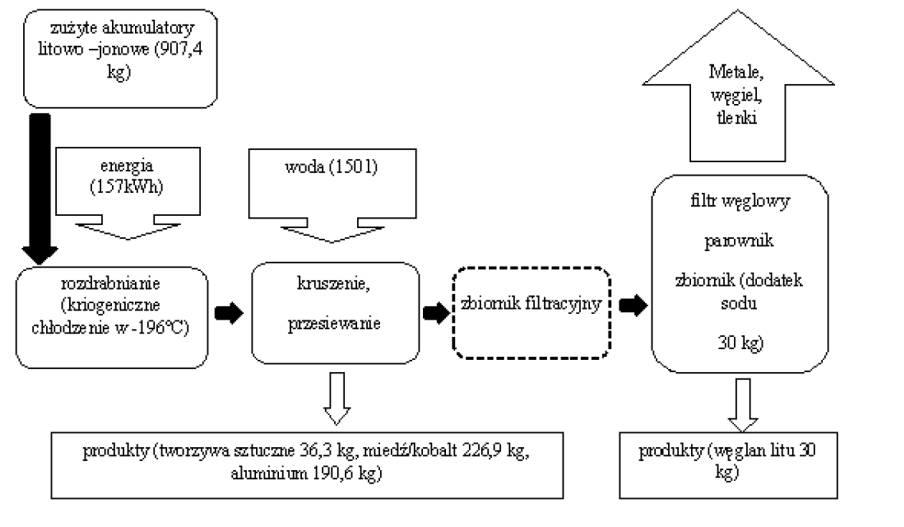
\includegraphics[width=9cm]{retriev.png}\cite{k20}
\end{frame}

\begin{frame}
	\frametitle{Procesy technologiczne}

	\begin{enumerate}
		\item Retriev - węglan litu i \ch{CO3} (zanurzanie w ciekłym azocie)
		\item Umicore - kobalt i nikiel
		\item Accurec - chlorek litu i stop kobaltu z magnanem (materiał katodowy)
		\item Recupryl - mielenie w atmosferze neutralnego gazu
		\item Batrec-Sumitomo
	\end{enumerate}

\end{frame}
%------------------------------------------------

\section{Podsumowanie}

\begin{frame}
	\frametitle{Podsumowanie}

\end{frame}

\begin{frame} % Use [allowframebreaks] to allow automatic splitting across slides if the content is too long
	\frametitle{Bibliografia}
	
	\begin{thebibliography}{99} % Beamer does not support BibTeX so references must be inserted manually as below, you may need to use multiple columns and/or reduce the font size further if you have many references
	\tiny	
	\bibitem{c05}
			Andrzej Czerwiński, 2005
			\newblock \emph{Akumulatory, baterie, ogniwa}
			
	\bibitem{b17}
			Christoph R. Birkl, 2017
			\newblock \emph{Degradation diagnostics for lithium ion cells}
	\bibitem{s19}
			Ewelina Sendek-Matysiak, 2019
			\newblock \emph{ Ocena baterii litowo-jonowych stosowanych w samochodach elektrycznych typu BEV pod względem bezpieczeństwa i wpływu na środowisko }
	\bibitem{m14}
			M. Bakierska, A. Chojnacka, 2014
			\newblock \emph{Akumulatory litowe jako współczesne systemy magazynowania energii}
	\bibitem{p17}
			Ch. Pillot, 2017
			\newblock \emph{The Rechargeable Battery Market and Main Trends 2016–2025.}
	\bibitem{c17}
			Chris Davies, 2017
			\newblock \emph{BMW's battery graveyard gives EV cast-offs a second life}
			https://www.slashgear.com/bmws-battery-graveyard-gives-ev-cast-offs-a-second-life-26505613/
	\bibitem{c22}
			Karolina Charzewska, 2022
			\newblock \emph{ Recykling akumulatorów litowo-jonowych na potrzeby gospodarki o obiegu zamkniętym }
	\bibitem{k20}
			Kamińska Ewa, Pawlak Piotr, 2020
			\newblock \emph{ Analiza ekobilansowa recyklingu zużytych litowo-jonowych akumulatorów samochodowych w technologii Retriev }
		\bibitem{s21}
			Su Chun, Chen Hongjing, Wen Zejun, 2021
			\newblock \emph{Prediction of remaining useful life for lithium-ion battery with multiple health indicators}
	\end{thebibliography}
\end{frame}

%----------------------------------------------------------------------------------------
%	CLOSING SLIDE
%----------------------------------------------------------------------------------------

\begin{frame}[plain] % The optional argument 'plain' hides the headline and footline
	\begin{center}
		{\Huge Dziękuję za uwagę :)}
		
		\bigskip\bigskip % Vertical whitespace
		
		{\LARGE Pytania?}
	\end{center}
\end{frame}

%----------------------------------------------------------------------------------------

\end{document} 
